\documentclass[10pt]{article}
\textheight = 21cm
\textwidth = 15cm
\topmargin = -0.5cm
\oddsidemargin = 1cm

\usepackage{amsmath}
\usepackage[utf8]{inputenc}
\usepackage[spanish]{babel}
\usepackage{graphicx}
\usepackage{fancyhdr}
\usepackage{epstopdf}
\usepackage{titling}
\usepackage{fancyvrb,fancybox,calc} 
\usepackage[svgnames]{xcolor} 
\usepackage{enumerate}
\usepackage{adjustbox}
\usepackage{tabu}
\usepackage{multicol}
\usepackage{float}
\usepackage{subcaption}
\usepackage[T1]{fontenc}
\usepackage{amsmath,amssymb}
\usepackage{geometry}

\newcommand{\HRule}{\rule{\linewidth}{0.5mm}}
\DeclareGraphicsExtensions{.pdf,.png,.jpg}

\parindent=0mm

\definecolor{light-gray}{gray}{0.94}
\definecolor{textgray}{gray}{0.5}
\newenvironment{verbcode}{\VerbatimEnvironment
  \begin{Sbox} \color{textgray}\scriptsize
  \begin{minipage}{\linewidth+2\fboxsep-2\fboxrule-12pt}    
  \begin{Verbatim}
}{\end{Verbatim}  
  \end{minipage}   
  \end{Sbox} \color{black}\normalsize
  \fcolorbox{black}{light-gray}{\TheSbox} 
} 

\begin{document}
\begin{center}

\textsc{\LARGE Sistemas de Control}\\[0.2cm]
\textsc{\Large Instituto Tecnológico de Buenos Aires}\\[0.2cm]

% Title
\HRule \\[0.2cm]
{ \huge \bfseries Entrega guía número 4 \\[0.2cm] }
\HRule \\[1cm]

\begin{multicols}{2}


% Integrantes
\columnbreak
{\raggedright
\large
\emph{Alumnos/as:} \ Bautista \textsc{Estrada} \\
\hspace*{2.5cm} Facundo \textsc{Garaguso Fernandez}\\
\hspace*{2.5cm} Joaquín \textsc{Basualdo}\\
}
\end{multicols}

\vspace{0.5cm}

\begin{adjustbox}{max width=\textwidth}
\renewcommand{\arraystretch}{1.5}
  \begin{tabular}{|l|c|}
    \hline
    \ \ \ Nota Final    &              \\ \hline \hline
    \ \ \ Firma y Fecha &              \\ \hline
  \end{tabular}
\end{adjustbox}

\end{center}

\vspace{0.2cm}

\pagestyle{fancy}
\headheight=60pt
\fancyhead[L]{Sistemas de Control - ITBA - 2026}        
\fancyhead[R]{Guia 4}

\newpage

\section*{Ejercicio 2}

\begin{figure}[H]
    \centering
    \includegraphics[width=\textwidth]{imagenes/Ej2.png}
\end{figure}

\vspace{0.4cm}

% -------------------------------------------------------------------------
% INCISO A + C
% -------------------------------------------------------------------------
\noindent{\Large\textbf{\textcircled{\normalsize a}}} + {\Large\textbf{\textcircled{\normalsize c}}}\hspace{0.2cm} \textbf{\textcolor{RoyalBlue}{Análisis de la condición de fase y de módulo}}

\begin{itemize}
    \item Calculo el aporte de fase de cada singularidad en $s = -1 + 2j$
\end{itemize}

\[
\angle (s + 55) = \arctan\left(\frac{2}{54}\right) = 2{,}12^{\circ}
\]

\[
\angle s = 180^{\circ} - \arctan\left(\frac{2}{1}\right) = 116{,}57^{\circ}
\]

\[
\angle (s + 2) = \arctan\left(\frac{2}{1}\right) = 63{,}43^{\circ}
\]

\[
\angle (s + 5) = \arctan\left(\frac{2}{4}\right) = 26{,}57^{\circ}
\]

\[
\sum \text{Fase} = 2{,}12^{\circ} - 116{,}57^{\circ} - 63{,}43^{\circ} - 26{,}57^{\circ} = -204{,}45^{\circ}
\]

\begin{itemize}
    \item Para cumplir la condición de fase ($-180^{\circ}$) falta aportar $24{,}45^{\circ}$ positivos, por lo que uso un controlador con un cero.
\end{itemize}

\[
\tan(24{,}45^{\circ}) = 0{,}4548 = \frac{2}{x}
\]

\[
x = 4{,}4 \longrightarrow \text{el cero se ubica en } s = -1 - 4{,}4 = -5{,}4
\]

\[
C(s) = K \cdot (s + 5{,}4)
\]



\begin{itemize}
    \item Saco la ganancia $K$ con la condición de módulo
\end{itemize}

\[
\left| \frac{0{,}1 \cdot K \cdot (s + 55) \cdot (s + 5{,}4)}{s \cdot (s + 2) \cdot (s + 5)} \right|_{s = -1 + 2j} = 1
\]

\[
\frac{0{,}1 \cdot K \cdot \sqrt{54^2 + 2^2} \cdot \sqrt{4{,}4^2 + 2^2}}{\sqrt{(-1)^2 + 2^2} \cdot \sqrt{1^2 + 2^2} \cdot \sqrt{4^2 + 2^2}} = 1
\]

\[
\frac{0{,}1 \cdot K \cdot 54{,}037 \cdot 4{,}833}{5 \cdot 4{,}472} = 1
\]

\[
1{,}168 \cdot K = 1 \longrightarrow K = 0{,}856
\]

\[
\fbox{$C(s) = 0{,}856 \cdot (s + 5{,}4)$}
\]


\begin{figure}[H]
    \centering
    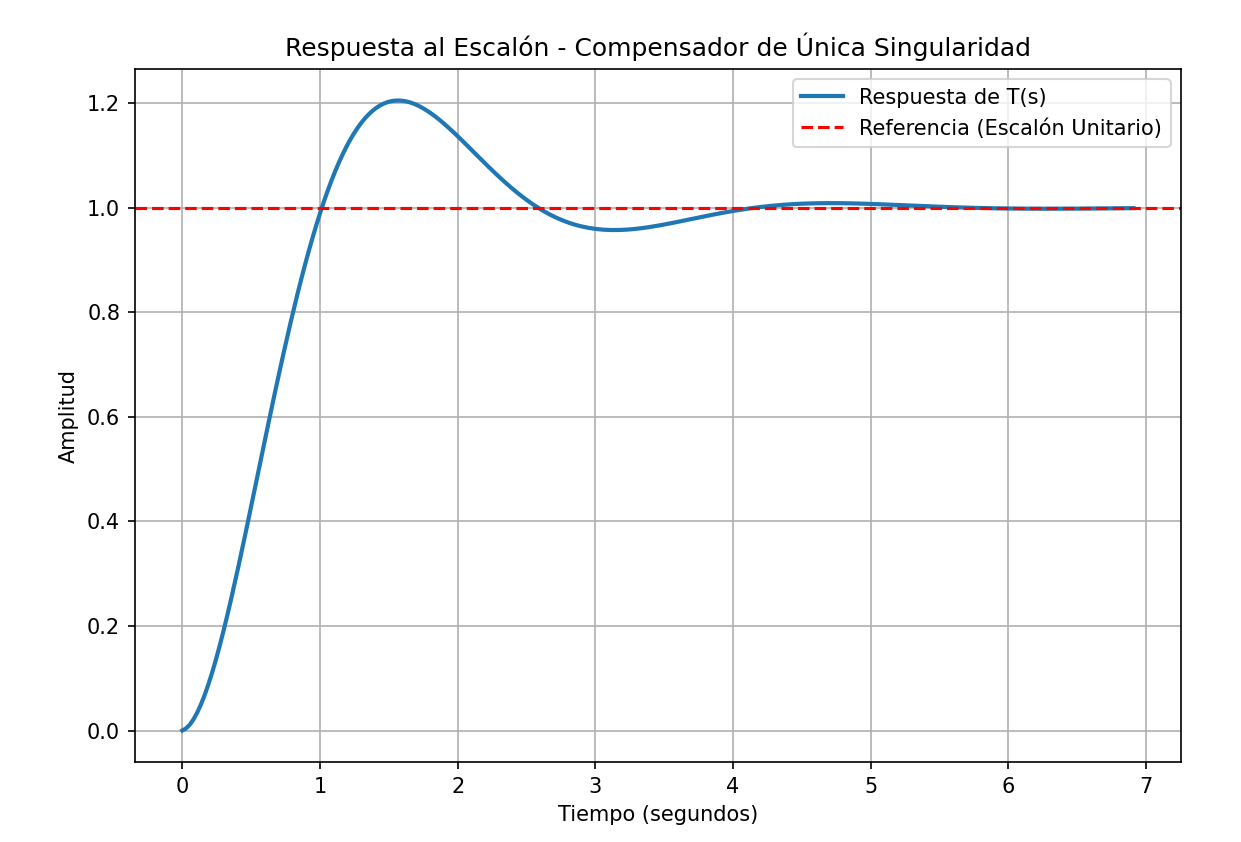
\includegraphics[width=\textwidth]{imagenes/unasing.png}
\end{figure}

\vspace{0.4cm}

% -------------------------------------------------------------------------
% INCISO D
% -------------------------------------------------------------------------
\noindent{\Large\textbf{\textcircled{\normalsize d}}}\hspace{0.2cm} \textbf{\textcolor{RoyalBlue}{Parámetros característicos}}

\[
-1 \pm 2j = -\xi \cdot \omega_n \pm j \cdot \omega_n \sqrt{1 - \xi^2} = -\xi \cdot \omega_n \pm j \cdot \omega_d
\]

\[
\xi \cdot \omega_n = 1 \qquad \omega_d = 2
\]

\begin{itemize}
    \item Saco el tiempo de establecimiento ($t_s$)
\end{itemize}

\[
t_s \approx \frac{4}{\xi \cdot \omega_n} = \frac{4}{1}
\]

\[
\fbox{$t_s \approx 4\text{ s}$}
\]

\begin{itemize}
    \item Saco el sobrepico ($M_p$)
\end{itemize}

\[
M_p = e^{\frac{-\pi \cdot \xi}{\sqrt{1 - \xi^2}}} = e^{\frac{-\pi \cdot \xi \cdot \omega_n}{\omega_d}} = e^{\frac{-\pi}{2}}
\]

\[
\fbox{$M_p = 0{,}2079$}
\]

\begin{itemize}
    \item Saco la $T(s)$
\end{itemize}

\[
T(s) = \frac{C(s) \cdot G(s)}{1 + C(s) \cdot G(s) \cdot H(s)} = \frac{0{,}0856 \cdot (s + 55) \cdot (s + 5{,}4)}{s \cdot (s + 2) \cdot (s + 5) + 0{,}0856 \cdot (s + 55) \cdot (s + 5{,}4)}
\]

\[
T(s) = \frac{0{,}0856 \, s^2 + 5{,}170 \, s + 25{,}42}{s^3 + 7{,}0856 \, s^2 + 15{,}170 \, s + 25{,}42}
\]

\[
T(s) = \frac{0{,}0856 \cdot (s + 55) \cdot (s + 5{,}4)}{(s^2 + 2s + 5) \cdot (s + 5{,}086)}
\]

\textit{Aparece un tercer polo en $-5{,}086$ y dos ceros.}


\begin{itemize}
    \item De la simulación: $M_p = 20{,}5$\,\% y $t_s = 3{,}73$ s.
    \item Los parámetros no se cumplen con exactitud, aunque la diferencia es muy chica. Las fórmulas son válidas para un sistema de orden 2 puro sin ceros, y $T(s)$ es de orden 3 con dos ceros.
    \item El polo en $-5{,}086$ queda muy cerca del cero en $-5{,}4$, por lo que casi se cancelan. El cero en $-55$ está muy alejado del eje imaginario. Por eso los polos $-1 \pm 2j$ son dominantes y la respuesta se parece mucho a la de un sistema de orden 2 puro.
    \item Además, $t_s \approx \frac{4}{\xi \cdot \omega_n}$ es una aproximación obtenida de la envolvente $e^{-\xi \cdot \omega_n \cdot t}$, por lo que ni siquiera un sistema de orden 2 puro da exactamente 4 s.
\end{itemize}
\vspace{0.4cm}

% -------------------------------------------------------------------------
% INCISO E
% -------------------------------------------------------------------------
\noindent{\Large\textbf{\textcircled{\normalsize e}}}\hspace{0.2cm} \textbf{\textcolor{RoyalBlue}{Método de la cancelación}}

\begin{itemize}
    \item Si cancelo el polo en $-5$ y el cero en $-55$, me queda un sistema de orden 2 tipo 1 con lugar de raíces entre $0$ y $-2$, que es lo que busco.
\end{itemize}

\[
C(s) = \frac{K \cdot (s + 5)}{(s + 55)}
\]

\[
C(s) \cdot G(s) \cdot H(s) = \frac{0{,}1 \cdot (s + 55)}{s \cdot (s + 2) \cdot (s + 5)} \cdot \frac{K \cdot (s + 5)}{(s + 55)} = \frac{0{,}1 \cdot K}{s \cdot (s + 2)}
\]

\begin{itemize}
    \item Saco la ganancia $K$ con la condición de módulo
\end{itemize}

\[
\left| \frac{0{,}1 \cdot K}{s \cdot (s + 2)} \right|_{s = -1 + 2j} = 1
\]

\[
\frac{0{,}1 \cdot K}{\sqrt{(-1)^2 + 2^2} \cdot \sqrt{1^2 + 2^2}} = \frac{0{,}1 \cdot K}{5} = 1 \longrightarrow K = 50
\]

\[
\fbox{$C(s) = \frac{50 \cdot (s + 5)}{(s + 55)}$}
\]


\vspace{0.4cm}

% -------------------------------------------------------------------------
% INCISO F
% -------------------------------------------------------------------------
\noindent{\Large\textbf{\textcircled{\normalsize f}}}\hspace{0.2cm} \textbf{\textcolor{RoyalBlue}{Conclusión}}

\begin{itemize}
    \item Saco la $T(s)$
\end{itemize}

\[
T(s) = \frac{\frac{5}{s \cdot (s + 2)}}{1 + \frac{5}{s \cdot (s + 2)}} = \frac{5}{s^2 + 2s + 5}
\]

\[
\omega_n = \sqrt{5} = 2{,}236 \qquad \xi = \frac{1}{\sqrt{5}} = 0{,}447
\]

\begin{figure}[H]
    \centering
    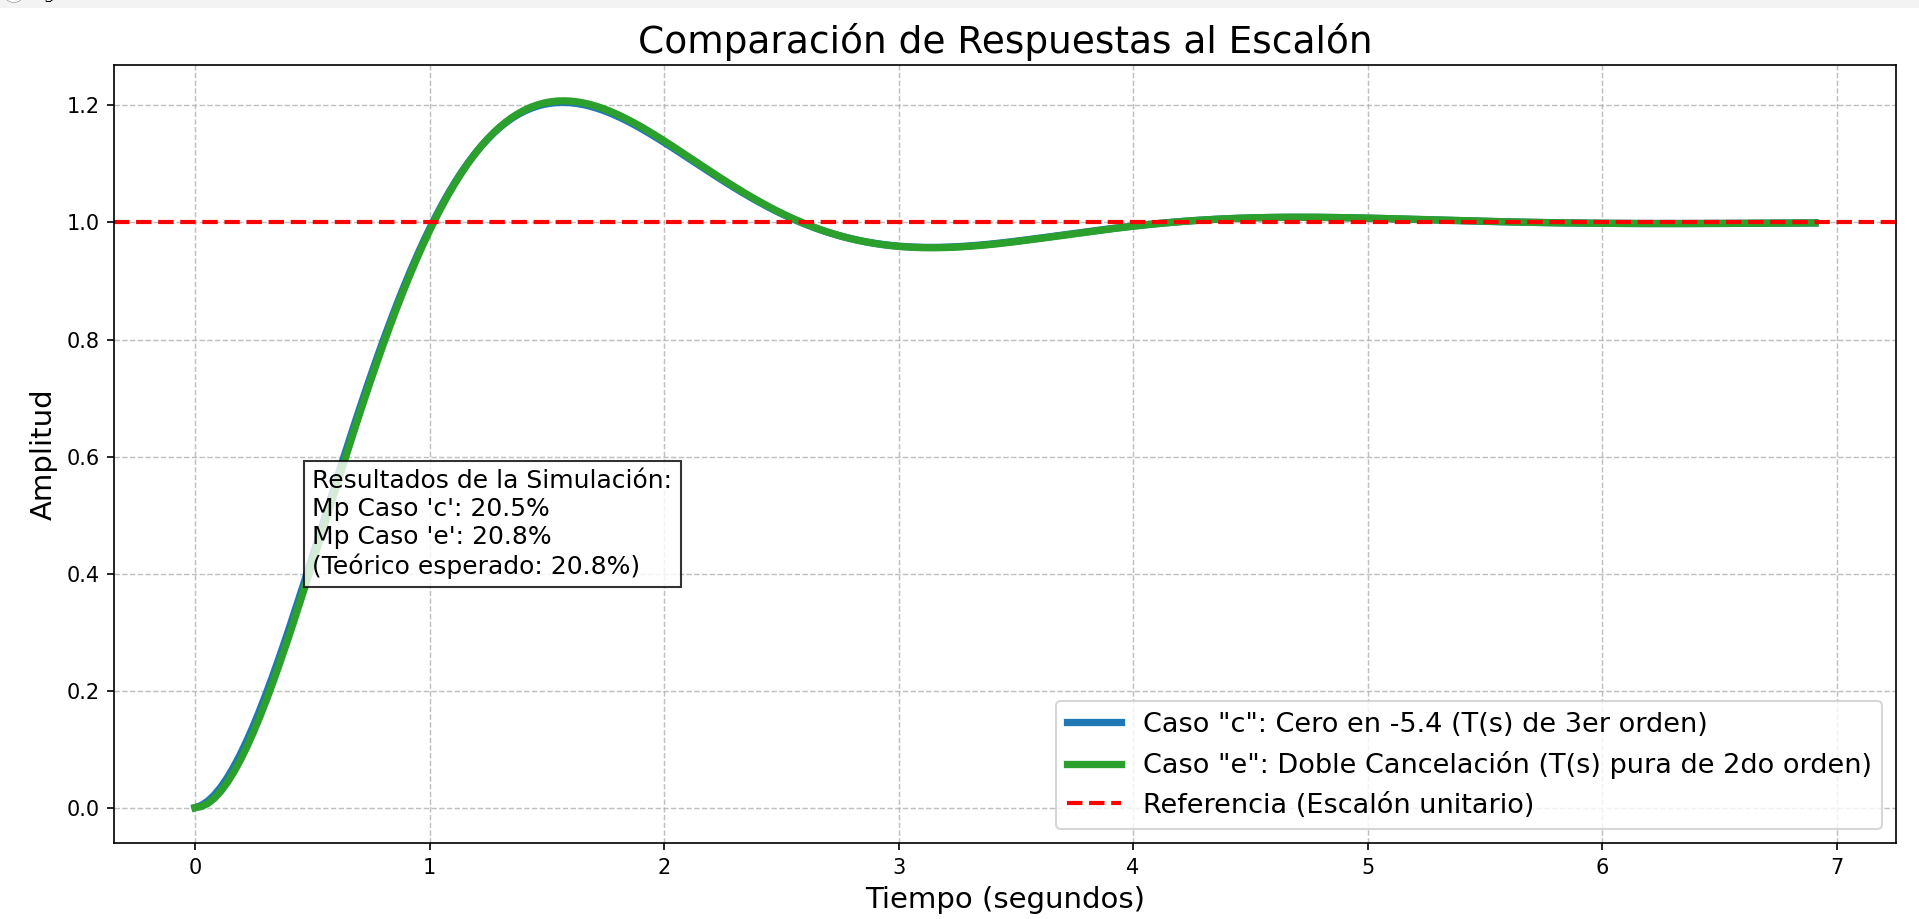
\includegraphics[width=\textwidth]{imagenes/dosing.png}
\end{figure}


\begin{itemize}
    \item De la simulación: $M_p = 20{,}8$\,\% y $t_s = 3{,}74$ s.
    \item Ahora $T(s)$ es un sistema de orden 2 puro, por lo que el sobrepico coincide con el teórico ($M_p = 20{,}79$\,\%). La diferencia en $t_s$ ($3{,}74$ s contra $4$ s) se debe solo a que la fórmula $t_s \approx \frac{4}{\xi \cdot \omega_n}$ es una aproximación.
    \item Esto confirma que la diferencia en el sobrepico del inciso d ($20{,}5$\,\%) se debía al tercer polo y a los ceros de $T(s)$.
    \item Ambos diseños dan respuestas prácticamente iguales. En el inciso c el tercer polo ($-5{,}086$) y el cero agregado ($-5{,}4$) quedan tan cerca que casi se cancelan, y el cero en $-55$ está muy alejado. En la práctica, el diseño c se comporta como si hubiera hecho una cancelación.
    \item El compensador del inciso c es un cero puro, $C(s) = 0{,}856 \cdot (s + 5{,}4)$. No es físicamente realizable porque tiene más ceros que polos, y amplifica el ruido de alta frecuencia. Para implementarlo habría que agregarle un polo alejado.
    \item El compensador del inciso e es una red de adelanto, que tiene igual cantidad de polos y ceros, así que sí es realizable. Su desventaja es que depende de que la cancelación sea exacta.
\end{itemize}

\vspace{0.4cm}

% -------------------------------------------------------------------------
% INCISO G
% -------------------------------------------------------------------------
\noindent{\Large\textbf{\textcircled{\normalsize g}}}\hspace{0.2cm} \textbf{\textcolor{RoyalBlue}{Routh-Hurwitz del inciso c}}

\[
1 + C(s) \cdot G(s) \cdot H(s) = 1 + \frac{0{,}1 \cdot K \cdot (s + 55) \cdot (s + 5{,}4)}{s \cdot (s + 2) \cdot (s + 5)} = 0
\]

\[
s^3 + 7s^2 + 10s + 0{,}1 \cdot K \cdot (s^2 + 60{,}4\,s + 297) = 0
\]

\[
s^3 + (7 + 0{,}1K) \, s^2 + (10 + 6{,}04K) \, s + 29{,}7K = 0
\]

\[
\begin{array}{c|cc}
s^3 & 1 & 10 + 6{,}04K \\
s^2 & 7 + 0{,}1K & 29{,}7K \\
s^1 & b_1 & 0 \\
s^0 & 29{,}7K &
\end{array}
\]

\[
b_1 = \frac{(7 + 0{,}1K) \cdot (10 + 6{,}04K) - 29{,}7K}{7 + 0{,}1K} = \frac{0{,}604K^2 + 13{,}58K + 70}{7 + 0{,}1K} > 0
\]

\[
\fbox{Estable $\forall \, K > 0$}
\]

\noindent{\Large\textbf{\textcircled{\normalsize g}}}\hspace{0.2cm} \textbf{\textcolor{RoyalBlue}{Routh-Hurwitz del inciso e}}

\[
1 + C(s) \cdot G(s) \cdot H(s) = 1 + \frac{0{,}1 \cdot (s + 55) \cdot K \cdot (s + 5)}{s \cdot (s + 2) \cdot (s + 5) \cdot (s + 55)} = 0
\]

\[
s^2 + 2s + 0{,}1K = 0
\]

\[
\begin{array}{c|cc}
s^2 & 1 & 0{,}1K \\
s^1 & 2 & 0 \\
s^0 & 0{,}1K &
\end{array}
\]

\[
\fbox{Estable $\forall \, K > 0$}
\]

\begin{itemize}
    \item Al aplicar Routh sobre el polinomio simplificado, los modos cancelados no aparecen. La ecuación característica completa es $(s + 5) \cdot (s + 55) \cdot (s^2 + 2s + 0{,}1K) = 0$, por lo que hay polos de lazo cerrado ocultos en $-5$ y $-55$.
\end{itemize}


% -------------------------------------------------------------------------
% EJERCICIO 5
% -------------------------------------------------------------------------

\section*{Ejercicio 5}

\begin{figure}[H]
    \centering
    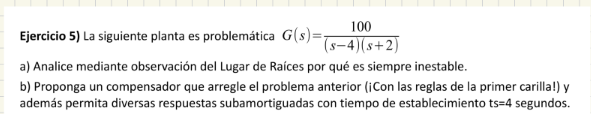
\includegraphics[width=\textwidth]{imagenes/Ej5.png}
\end{figure}

\vspace{0.4cm}

% -------------------------------------------------------------------------
% INCISO A
% -------------------------------------------------------------------------
\noindent{\Large\textbf{\textcircled{\normalsize a}}}\hspace{0.2cm} \textbf{\textcolor{RoyalBlue}{Lugar de raíces}}

\begin{itemize}
    \item La planta tiene dos polos, en $+4$ y en $-2$, y ningún cero. Pertenece al lugar de raíces el tramo del eje real entre $-2$ y $+4$.
    \item Calculo el centroide y los ángulos de las asíntotas
\end{itemize}

\[
\sigma = \frac{\sum \mathrm{polos} - \sum \mathrm{ceros}}{n_p - n_z} = \frac{(4 - 2) - 0}{2 - 0} = 1
\]

\[
\theta = \frac{(2k + 1) \cdot 180^{\circ}}{2 - 0} \longrightarrow \theta_1 = 90^{\circ} \qquad \theta_2 = 270^{\circ}
\]

\begin{itemize}
    \item Las ramas se encuentran en el punto de separación $\sigma = 1$ y desde ahí suben y bajan por la recta vertical $\sigma = 1$.
\end{itemize}

\begin{figure}[H]
    \centering
    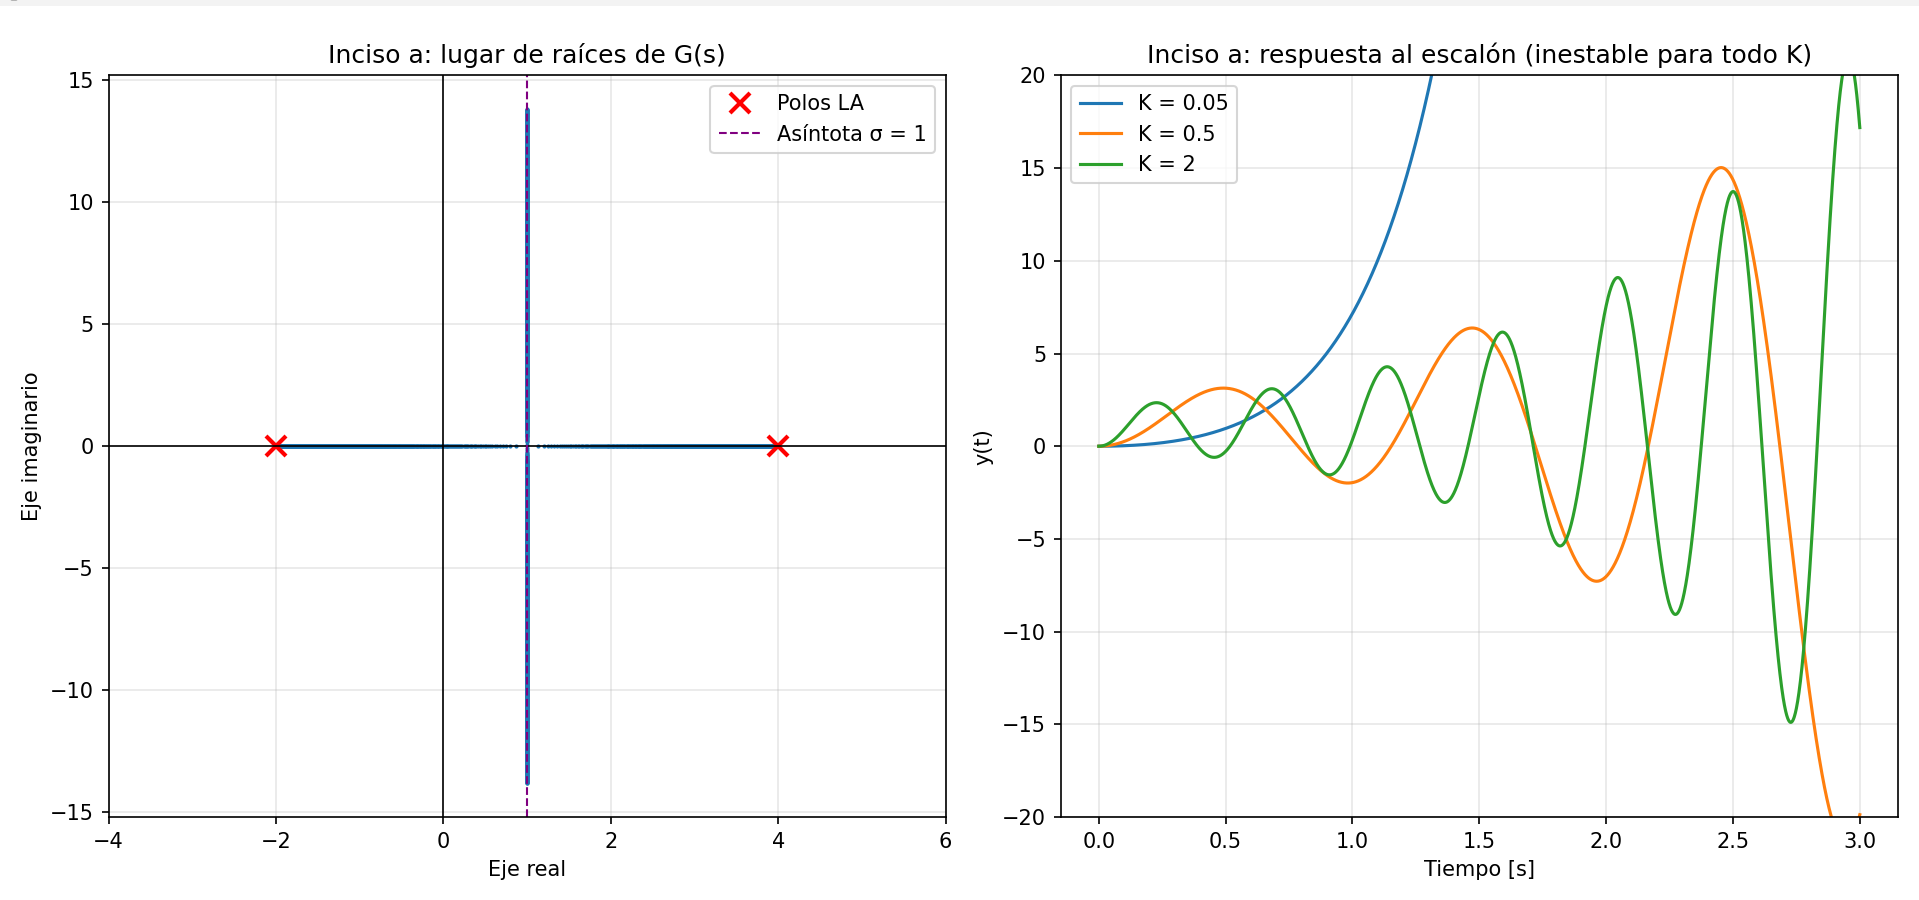
\includegraphics[width=\textwidth]{imagenes/Ej5a.png}
\end{figure}

\begin{itemize}
    \item El sistema siempre será inestable. Para $K$ chico los polos son reales y uno de ellos queda entre $+1$ y $+4$. Cuando se separan, quedan complejos conjugados con parte real $+1$. En ambos casos siempre hay al menos un polo en el semiplano derecho.
    \item Lo confirmo con Routh. La ecuación característica es
\end{itemize}

\[
1 + K \cdot G(s) = 0 \longrightarrow s^2 - 2s + (100K - 8) = 0
\]

\begin{itemize}
    \item El coeficiente de $s$ es $-2$, que es negativo y no depende de $K$. Por lo tanto hay un cambio de signo en la primera columna de Routh para cualquier $K$.
\end{itemize}

\[
\fbox{Inestable $\forall \, K$}
\]

\vspace{0.4cm}

% -------------------------------------------------------------------------
% INCISO B
% -------------------------------------------------------------------------
\noindent{\Large\textbf{\textcircled{\normalsize b}}}\hspace{0.2cm} \textbf{\textcolor{RoyalBlue}{Diseño del compensador}}

\begin{itemize}
    \item \textbf{Regla 1:} con ganancia no se puede resolver, por lo demostrado en el inciso anterior.
    \item \textbf{Regla 4:} el compensador no debe tener singularidades en el semiplano derecho y mucho menos cancelarlas. No puedo tocar el polo en $+4$.
    \item Saco la parte real de los polos de lazo cerrado
\end{itemize}

\[
t_s = 4 \, \mathrm{s} = \frac{4}{\xi \cdot \omega_n} \longrightarrow \xi \cdot \omega_n = 1
\]

\begin{itemize}
    \item Los polos deben tener parte real $-1$. Para que haya diversas respuestas subamortiguadas con el mismo $t_s$, el lugar de raíces tiene que ser una recta vertical en $\sigma = -1$.
    \item Con dos polos y ningún cero, la recta vertical pasa por el centroide. Cancelo el polo en $-2$ (permitido por estar en el semiplano izquierdo) y agrego un polo en $-6$ para que el centroide sea $-1$:
\end{itemize}

\[
\sigma = \frac{4 + (-6)}{2} = -1
\]

\[
\fbox{$C(s) = \frac{K \cdot (s + 2)}{(s + 6)}$}
\]

\begin{itemize}
    \item El compensador es una red de adelanto: tiene igual cantidad de polos y ceros, por lo que es físicamente realizable. Además todas sus singularidades son reales y están en el semiplano izquierdo, cumpliendo las reglas 3 y 4.
    \item Saco la $T(s)$
\end{itemize}

\[
T(s) = \frac{G(s) \cdot C(s)}{1 + G(s) \cdot C(s)} = \frac{\frac{100 \cdot K}{(s - 4) \cdot (s + 6)}}{1 + \frac{100 \cdot K}{(s - 4) \cdot (s + 6)}} = \frac{100 \cdot K}{s^2 + 2s + (100K - 24)}
\]

\begin{itemize}
    \item Comparo con la forma estándar $s^2 + 2 \xi \omega_n s + \omega_n^2$
\end{itemize}

\[
2 \cdot \xi \cdot \omega_n = 2 \longrightarrow \xi \cdot \omega_n = 1
\]

\[
\omega_n = \sqrt{100K - 24} \qquad \xi = \frac{1}{\omega_n}
\]

\begin{itemize}
    \item El término en $s$ no depende de $K$, por lo que la parte real de los polos queda fija en $-1$. Al aumentar $K$ aumenta $\omega_n$, disminuye $\xi$ y aumenta el sobrepico, pero $t_s$ se mantiene.
\end{itemize}

\begin{itemize}
    \item \textbf{Routh} para ver la estabilidad (Regla 5)
\end{itemize}

\[
P(s) = s^2 + 2s + (100K - 24)
\]

\[
\begin{array}{c|cc}
s^2 & 1 & 100K - 24 \\
s^1 & 2 & 0 \\
s^0 & 100K - 24 &
\end{array}
\]

\[
\fbox{Estable $\forall \, K > 0{,}24$}
\]

\begin{itemize}
    \item Saco a partir de qué $K$ el sistema es subamortiguado. Las ramas pasan de reales a complejas en el punto de separación $s = -1$. Aplico la condición de módulo:
\end{itemize}

\[
\left| \frac{100 \cdot K}{(s - 4) \cdot (s + 6)} \right|_{s = -1} = 1
\]

\[
\frac{100 \cdot K}{5 \cdot 5} = 1 \longrightarrow K = 0{,}25
\]

\begin{itemize}
    \item Lo verifico con el discriminante de $P(s)$:
\end{itemize}

\[
4 - 4 \cdot (100K - 24) < 0 \longrightarrow 100K - 24 > 1 \longrightarrow K > 0{,}25
\]

\[
\fbox{Subamortiguado $\forall \, K > 0{,}25$}
\]

\begin{itemize}
    \item $0{,}24 < K < 0{,}25$: estable pero sobreamortiguado. Los polos son reales y no se cumple $t_s = 4$ s.
    \item $K = 0{,}25$: críticamente amortiguado, polo doble en $-1$.
    \item $K > 0{,}25$: subamortiguado, polos en $-1 \pm j \omega_d$. Se cumple $t_s \approx 4$ s para cualquier $K$.
    \item \textbf{Regla 8:} el polo cancelado en $-2$ sigue estando en la ecuación característica completa, $(s + 2) \cdot (s^2 + 2s + 100K - 24) = 0$. No genera problemas porque está en el semiplano izquierdo.
\end{itemize}

\begin{figure}[H]
    \centering
    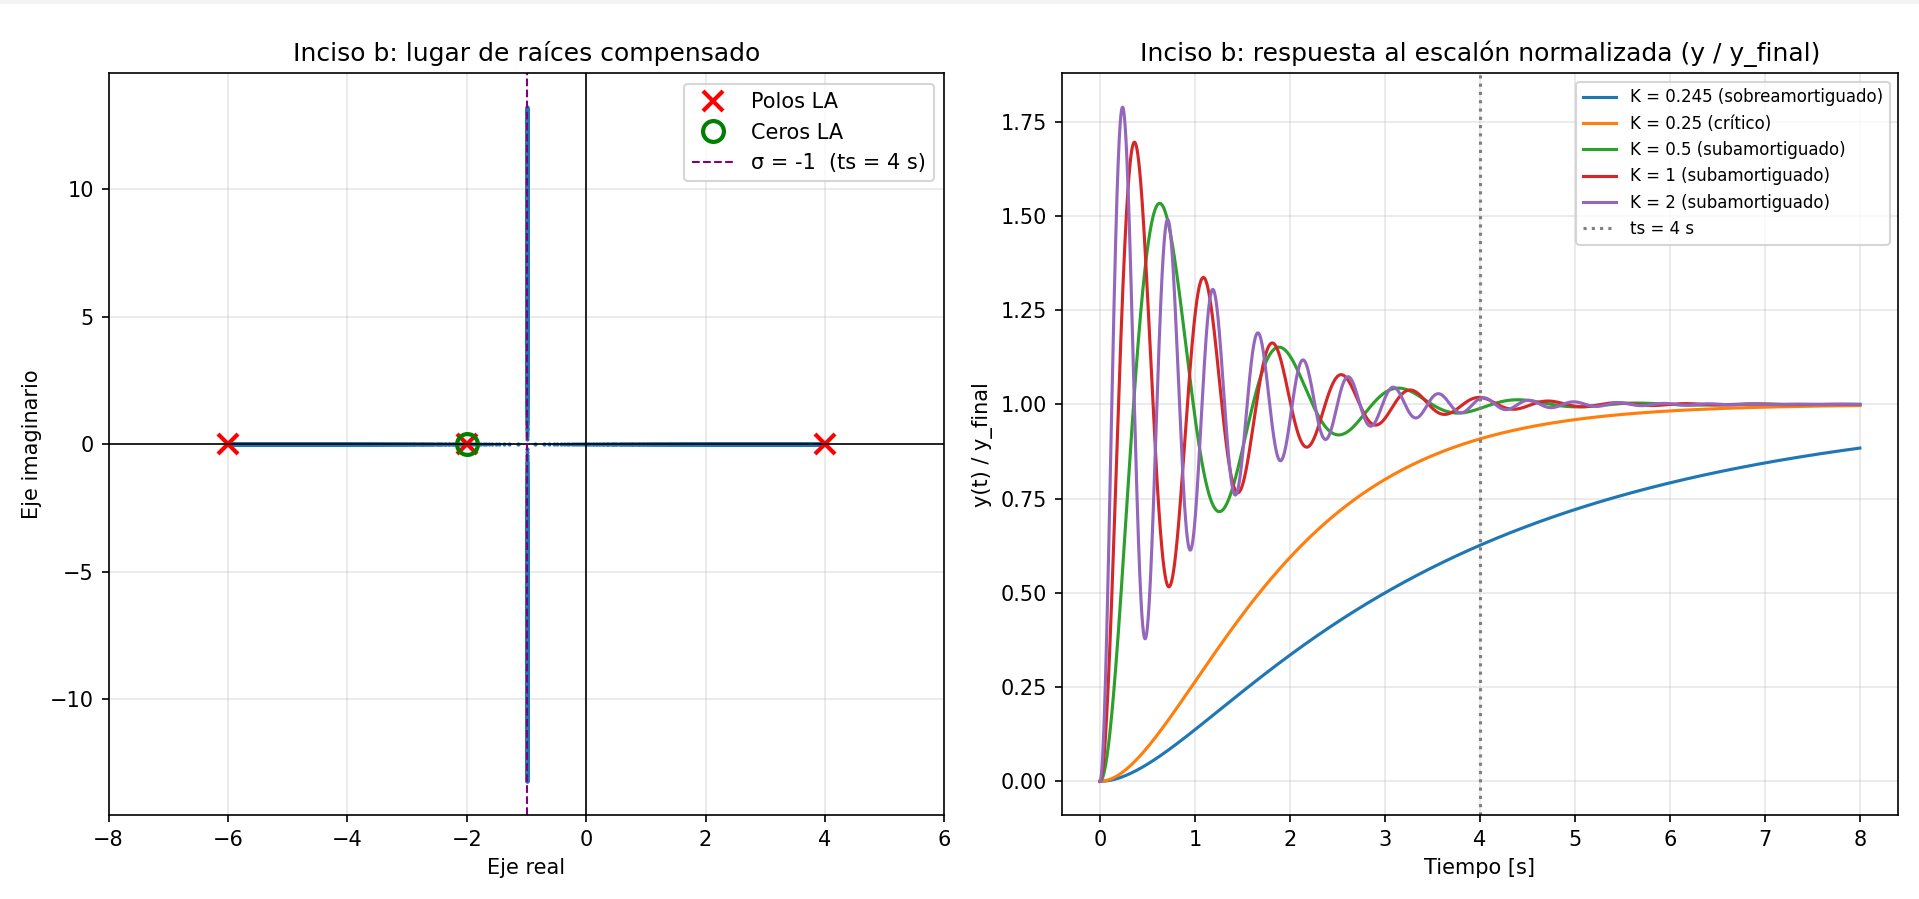
\includegraphics[width=\textwidth]{imagenes/Ej5b.png}
\end{figure}

\begin{itemize}
    \item De la simulación: con $K = 0{,}5$, $K = 1$ y $K = 2$ se obtienen $t_s = 3{,}88$ s, $3{,}71$ s y $3{,}83$ s respectivamente, con sobrepicos de $53{,}3$\,\%, $69{,}6$\,\% y $78{,}9$\,\%. El sobrepico cambia con $K$ pero el tiempo de establecimiento se mantiene cerca de 4 s, como se buscaba.
    \item Con $K = 0{,}245$ (sobreamortiguado) y $K = 0{,}25$ (crítico) el sistema es estable pero tarda más que 4 s, ya que los polos no tienen parte real $-1$.
\end{itemize}



\section*{Ejercicio 12 -- Incubadora neonatal}

\begin{figure}[H]
    \centering
    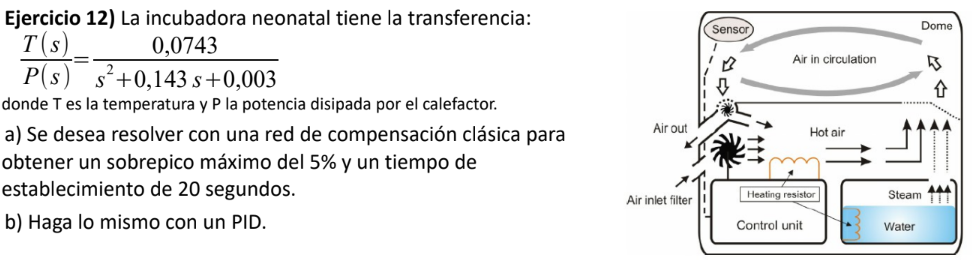
\includegraphics[width=\textwidth]{imagenes/Ej12.png}
\end{figure}


La incubadora neonatal presenta la siguiente
función de transferencia:

\begin{equation}
    G(s)=\frac{T(s)}{P(s)}
    =\frac{0.0743}{s^2+0.143s+0.003}
\end{equation}

donde $T(s)$ representa la temperatura y
$P(s)$ la potencia disipada por el calefactor.

Se desea obtener:
\[
MP=5\%, \qquad t_s=20\,s
\]

Se considera realimentación unitaria:

\[
H(s)=1
\]

\subsection*{Cálculos preliminares}

Para un sistema de segundo orden, el
sobrepico está relacionado con el
coeficiente de amortiguamiento mediante:

\begin{equation}
    MP=e^{-\frac{\pi\zeta}
    {\sqrt{1-\zeta^2}}}
\end{equation}

Reemplazando:

\[
0.05=e^{-\frac{\pi\zeta}
{\sqrt{1-\zeta^2}}}
\]

Aplicando logaritmo natural:

\[
\ln(0.05)=
-\frac{\pi\zeta}{\sqrt{1-\zeta^2}}
\]

Despejando:

\begin{equation}
    \boxed{\zeta=0.6901}
\end{equation}

Utilizamos la aproximación del tiempo
de establecimiento al $2\%$:

\begin{equation}
    t_s\simeq\frac{4}{\zeta\omega_n}
\end{equation}

Como $t_s=20\,s$:

\[
20=\frac{4}{0.6901\omega_n}
\]

Por lo tanto:

\begin{equation}
    \boxed{\omega_n=0.2898\ rad/s}
\end{equation}

Los polos deseados son:

\[
s_{d1,2}=
-\zeta\omega_n
\pm j\omega_n\sqrt{1-\zeta^2}
\]

\begin{equation}
    \boxed{s_d=-0.2\pm j0.2097}
\end{equation}

Factorizamos el denominador de la planta:

\[
s^2+0.143s+0.003=(s+a)(s+b)
\]

Resolviendo la ecuación cuadrática:

\[
a=0.0255408,
\qquad b=0.1174592
\]

Por lo tanto:

\begin{equation}
    \boxed{
    G(s)=\frac{0.0743}
    {(s+0.0255408)(s+0.1174592)}
    }
\end{equation}

% ========================================

\section*{Inciso a) Compensación clásica}

Se desea diseñar un compensador clásico
formado por un polo, un cero y una ganancia.

Su estructura es:

\begin{equation}
    \boxed{
    C_a(s)=K\frac{s+z}{s+p}
    }
\end{equation}

\subsection*{1. Elección de la estructura}

Se utilizará el método de cancelación de
una singularidad estable de la planta.

Elegimos el cero del compensador para
cancelar el polo ubicado en:

\[
s=-0.1174592
\]

Por lo tanto:

\[
z=0.1174592
\]

El compensador resulta:

\[
C_a(s)=K\frac{s+0.1174592}{s+p}
\]

La transferencia de lazo abierto es:

\[
L_a(s)=C_a(s)G(s)H(s)
\]

\[
L_a(s)=
K\frac{s+0.1174592}{s+p}
\frac{0.0743}
{(s+0.0255408)(s+0.1174592)}
\]

Cancelando la singularidad:

\begin{equation}
    \boxed{
    L_a(s)=
    \frac{0.0743K}
    {(s+0.0255408)(s+p)}
    }
\end{equation}

Como la singularidad cancelada pertenece
al semiplano izquierdo, la cancelación
no introduce un modo interno inestable.

\subsection*{2. Condición de fase}

Para que los polos deseados pertenezcan
al Lugar de Raíces, debe cumplirse:

\begin{equation}
    \angle L_a(s_d)=-180^\circ
\end{equation}

Trabajamos con el polo deseado:

\[
s_d=-0.2+j0.2097
\]

El ángulo aportado por el polo de
la planta es:

\[
s_d+0.0255408
=
-0.1744592+j0.2097
\]

Por lo tanto:

\[
\phi_1=
180^\circ-
\tan^{-1}
\left(
\frac{0.2097}{0.1744592}
\right)
\]

\begin{equation}
    \boxed{\phi_1\simeq129.75^\circ}
\end{equation}

El polo del compensador debe aportar
el ángulo restante:

\[
\phi_p=180^\circ-129.75^\circ
\]

\begin{equation}
    \boxed{\phi_p=50.25^\circ}
\end{equation}

Utilizando geometría en el plano complejo:

\[
\tan(50.25^\circ)
=
\frac{0.2097}{p-0.2}
\]

Despejando:

\[
p=0.2+
\frac{0.2097}{\tan(50.25^\circ)}
\]

\begin{equation}
    \boxed{p\simeq0.37446}
\end{equation}

De esta forma, el compensador presenta
un polo en:

\[
s=-0.37446
\]

\subsection*{3. Condición de módulo}

Debe cumplirse:

\begin{equation}
    |L_a(s_d)|=1
\end{equation}

Por lo tanto:

\[
\left|
\frac{0.0743K}
{(s_d+0.0255408)(s_d+0.37446)}
\right|=1
\]

Despejando:

\[
K=
\frac{
|s_d+0.0255408|
|s_d+0.37446|
}{0.0743}
\]

Evaluando en el punto deseado:

\begin{equation}
    \boxed{K\simeq1.0017}
\end{equation}

\subsection*{4. Compensador obtenido}

Finalmente:

\begin{equation}
    \boxed{
    C_a(s)=
    1.0017
    \frac{s+0.1174592}{s+0.37446}
    }
\end{equation}

Se obtuvo una red de adelanto de fase,
ya que su cero se encuentra más cerca
del origen que su polo.

\subsection*{5. Transferencia a lazo cerrado}

La transferencia a lazo cerrado es:

\[
T_a(s)=\frac{L_a(s)}{1+L_a(s)}
\]

Reemplazando:

\[
T_a(s)=
\frac{0.0743K}
{(s+0.0255408)(s+0.37446)+0.0743K}
\]

Desarrollando y reemplazando la ganancia:

\begin{equation}
    \boxed{
    T_a(s)=
    \frac{0.074426}
    {s^2+0.4s+0.08399}
    }
\end{equation}

Comparando con el denominador
característico de segundo orden:

\[
s^2+2\zeta\omega_ns+\omega_n^2
\]

se verifica que:

\[
2\zeta\omega_n=0.4
\]

\[
\omega_n^2=0.08399
\]

Por lo tanto:

\[
\zeta=0.6901
\]

\[
\omega_n=0.2898\ rad/s
\]

Los polos de lazo cerrado son:

\begin{equation}
    \boxed{
    s_{1,2}=-0.2\pm j0.2097
    }
\end{equation}

\subsection*{6. Verificación temporal y estabilidad}

El sobrepico es:

\[
MP=
e^{-\frac{\pi\zeta}{\sqrt{1-\zeta^2}}}
\]

\begin{equation}
    \boxed{MP=5\%}
\end{equation}

El tiempo de establecimiento aproximado
al $2\%$ es:

\[
t_s\simeq\frac{4}{\zeta\omega_n}
\]

\begin{equation}
    \boxed{t_s\simeq20\,s}
\end{equation}

Además, ambos polos de lazo cerrado
poseen parte real negativa, por lo
que el sistema es estable.

El polo cancelado también pertenece
al semiplano izquierdo.

La ganancia estática es:

\[
T_a(0)=
\frac{0.074426}{0.08399}
\simeq0.88613
\]

Por lo tanto, el error estacionario
ante un escalón unitario es:

\[
e_{ss}=1-T_a(0)
\]

\begin{equation}
    \boxed{e_{ss}\simeq0.11387}
\end{equation}

Existe un error estacionario aproximado
del $11.39\%$, aunque esto no contradice
lo solicitado en el enunciado.

% ========================================

\section*{Inciso b) Compensación mediante PID}

Se desea resolver el mismo problema
utilizando un controlador PID.

La estructura general es:

\begin{equation}
C_{PID}(s)=K_P+\frac{K_I}{s}+K_Ds
\end{equation}

Equivalentemente:

\begin{equation}
\boxed{
C_{PID}(s)=
K\frac{(s+z_1)(s+z_2)}{s}
}
\end{equation}

\subsection*{1. Elección de la estructura}

Elegimos uno de los ceros del PID para
cancelar un polo estable de la planta:

\[
z_1=0.0255408
\]

Por lo tanto:

\[
C_{PID}(s)=
K\frac{(s+0.0255408)(s+z_2)}{s}
\]

La transferencia de lazo abierto es:

\[
L_b(s)=C_{PID}(s)G(s)
\]

\[
L_b(s)=
K\frac{(s+0.0255408)(s+z_2)}{s}
\frac{0.0743}
{(s+0.0255408)(s+0.1174592)}
\]

Cancelando:

\begin{equation}
\boxed{
L_b(s)=
\frac{0.0743K(s+z_2)}
{s(s+0.1174592)}
}
\end{equation}

\subsection*{2. Condición de fase}

Para que el punto deseado pertenezca
al Lugar de Raíces:

\[
\angle L_b(s_d)=-180^\circ
\]

Trabajamos con:

\[
s_d=-0.2+j0.2097
\]

Calculamos el aporte del polo
ubicado en el origen:

\[
\phi_1=
180^\circ-
\tan^{-1}
\left(\frac{0.2097}{0.2}\right)
\]

\begin{equation}
\boxed{\phi_1=133.64^\circ}
\end{equation}

El aporte del segundo polo es:

\[
s_d+0.1174592=
-0.0825408+j0.2097
\]

\[
\phi_2=
180^\circ-
\tan^{-1}
\left(
\frac{0.2097}{0.0825408}
\right)
\]

\begin{equation}
\boxed{\phi_2=111.48^\circ}
\end{equation}

La suma de ángulos de los polos es:

\[
\sum\phi_p=
133.64^\circ+111.48^\circ
\]

\[
\boxed{\sum\phi_p=245.12^\circ}
\]

Por lo tanto, el cero restante
debe aportar:

\[
\phi_z=245.12^\circ-180^\circ
\]

\begin{equation}
\boxed{\phi_z=65.12^\circ}
\end{equation}

Aplicando geometría:

\[
\tan(65.12^\circ)
=
\frac{0.2097}{z_2-0.2}
\]

Despejando:

\[
z_2=
0.2+\frac{0.2097}{\tan(65.12^\circ)}
\]

\begin{equation}
\boxed{z_2=0.29727}
\end{equation}

\subsection*{3. Condición de módulo}

Debe cumplirse:

\begin{equation}
|L_b(s_d)|=1
\end{equation}

Por lo tanto:

\[
\left|
\frac{
0.0743K(s_d+0.29727)
}{
s_d(s_d+0.1174592)
}
\right|=1
\]

Despejando:

\[
K=
\frac{
|s_d|\,|s_d+0.1174592|
}{
0.0743|s_d+0.29727|
}
\]

Evaluando en el punto deseado:

\begin{equation}
\boxed{K=3.8027}
\end{equation}

\subsection*{4. Controlador PID obtenido}

Finalmente:

\begin{equation}
\boxed{
C_{PID}(s)=
3.8027
\frac{
(s+0.0255408)(s+0.29727)
}{s}
}
\end{equation}

Se obtuvo un controlador PID completo,
formado por:

\begin{itemize}
    \item Un polo en el origen.
    \item Un cero en $s=-0.0255408$.
    \item Un cero en $s=-0.29727$.
    \item Una ganancia $K=3.8027$.
\end{itemize}

\subsection*{5. Transferencia a lazo cerrado}

La transferencia a lazo cerrado es:

\[
T_b(s)=\frac{L_b(s)}{1+L_b(s)}
\]

Reemplazando:

\[
T_b(s)=
\frac{
0.0743K(s+0.29727)
}{
s(s+0.1174592)+0.0743K(s+0.29727)
}
\]

Desarrollando:

\begin{equation}
\boxed{
T_b(s)=
\frac{0.28254(s+0.29727)}
{s^2+0.4s+0.08399}
}
\end{equation}

Los polos de lazo cerrado son:

\begin{equation}
\boxed{
s_{1,2}=-0.2\pm j0.2097
}
\end{equation}

De esta manera se verifica que los
polos del sistema compensado coinciden
con los polos deseados.

Utilizando las relaciones aproximadas
de segundo orden asociadas a los polos:

\[
\boxed{\zeta=0.6901}
\]

\[
\boxed{\omega_n=0.2898\ rad/s}
\]

\[
MP_{\mathrm{aprox}}
=e^{-\frac{\pi\zeta}{\sqrt{1-\zeta^2}}}
\]

\begin{equation}
\boxed{MP_{\mathrm{aprox}}=5\%}
\end{equation}

Y para el tiempo de establecimiento:

\[
t_s\simeq\frac{4}{\zeta\omega_n}
\]

\begin{equation}
\boxed{t_s\simeq20\,s}
\end{equation}

Estas expresiones corresponden a
la aproximación de segundo orden
basada en los polos. No se evalúa
aquí la respuesta temporal completa,
que también depende del cero restante.

\subsection*{6. Parámetros del PID}

El controlador obtenido es:

\[
C_{PID}(s)=
3.8027
\frac{
(s+0.0255408)(s+0.29727)
}{s}
\]

Desarrollando el numerador:

\[
C_{PID}(s)=
K\frac{
s^2+(z_1+z_2)s+z_1z_2
}{s}
\]

Separando términos:

\[
C_{PID}(s)=
Ks+K(z_1+z_2)+\frac{Kz_1z_2}{s}
\]

Comparando con:

\[
C_{PID}(s)=K_P+\frac{K_I}{s}+K_Ds
\]

Obtenemos:

\[
K_D=K
\]

\[
K_P=K(z_1+z_2)
\]

\[
K_I=Kz_1z_2
\]

Reemplazando los valores:

\begin{equation}
\boxed{K_D=3.8027}
\end{equation}

\begin{equation}
\boxed{K_P\simeq1.2277}
\end{equation}

\begin{equation}
\boxed{K_I\simeq0.02887}
\end{equation}

Por lo tanto:

\begin{equation}
\boxed{
C_{PID}(s)=
1.2277+\frac{0.02887}{s}+3.8027s
}
\end{equation}

\subsection*{7. Verificación de estabilidad}

La ecuación característica es:

\[
s^2+0.4s+0.08399=0
\]

Como es un polinomio de segundo orden
con todos sus coeficientes positivos,
se cumple el criterio de Routh-Hurwitz.

Además, sus raíces son:

\[
s_{1,2}=-0.2\pm j0.2097
\]

El polo cancelado:

\[
s_3=-0.0255408
\]

también pertenece al semiplano izquierdo.

Por lo tanto, el sistema es estable.

\subsection*{8. Error de estado estacionario}

La transferencia de lazo abierto es:

\[
L_b(s)=
\frac{
0.28254(s+0.29727)
}{
s(s+0.1174592)
}
\]

Se observa que posee un polo en
el origen, por lo que el sistema
es de tipo 1.

Para una entrada escalón unitario:

\[
e_{ss}=
\lim_{s\to0}
\frac{1}{1+L_b(s)}
\]

Como:

\[
\lim_{s\to0}L_b(s)=\infty
\]

Se obtiene:

\begin{equation}
\boxed{e_{ss}=0}
\end{equation}

Esta es una ventaja adicional del
PID respecto del compensador clásico
utilizado en el inciso anterior.

\subsection*{Conclusión del inciso b)}

Se obtuvo el controlador PID:

\[
\boxed{
C_{PID}(s)=
3.8027
\frac{
(s+0.0255408)(s+0.29727)
}{s}
}
\]

Mediante el método de sumatoria
de ángulos y condición de módulo,
se ubicaron los polos de lazo cerrado
en las posiciones deseadas:

\[
\boxed{s_{1,2}=-0.2\pm j0.2097}
\]

Se verifica que el sistema es estable.

Además, la acción integral permite
eliminar el error de estado estacionario
frente a una entrada escalón.

\end{document}